% This is the code that generates the slides we'll use for this section.
% If you'd simply like to view the slides, please open slides.pdf


\documentclass[10pt, aspectratio=169]{beamer}

\makeatletter
  \def\beamer@calltheme#1#2#3{%
    \def\beamer@themelist{#2}
    \@for\beamer@themename:=\beamer@themelist\do
    {\usepackage[{#1}]{\beamer@themelocation/#3\beamer@themename}}}

  \def\usefolder#1{
    \def\beamer@themelocation{#1}
  }
  \def\beamer@themelocation{}

\usefolder{../../__resources__/beamer_theme}
\usetheme{nathan}

\addtobeamertemplate{navigation symbols}{}{%
    \usebeamerfont{footline}%
    \usebeamercolor[fg]{footline}%
    \hfill%
    \insertframenumber/\inserttotalframenumber
}

\title{Computational Decision Making for Regular People}
\subtitle{Debugging}
% \date{October 29, 2024}

\usepackage[font=tiny,labelfont=bf]{caption}
\usepackage{caption}
\captionsetup[figure]{labelformat=empty}

\usepackage{listings}
\usepackage{dirtree}

\usepackage{amssymb}% http://ctan.org/pkg/amssymb
\usepackage{pifont}% http://ctan.org/pkg/pifont
\newcommand{\cmark}{\ding{51}}%
\newcommand{\xmark}{\ding{55}}%

\begin{document}

\begin{frame}
    \maketitle
\end{frame}

\begin{frame}{Today's Outline}
    \begin{columns}
        \begin{column}{0.5\textwidth}
            \begin{enumerate}
                \item Types of Errors
                \item Python Traceback
                \item Math Modeling (Errors)
                \item How to handle "Unbounded" Results
                \item How to handle "Infeasible" Results
            \end{enumerate}
        \end{column}
        \begin{column}{0.5\textwidth}
            \begin{figure}
                \begin{figure}
                    \includegraphics[width=0.80\linewidth]{Frustrated.png}
                    \caption{This image was created with the assistance of DALL·E 3}
                \end{figure}
            \end{figure}
        \end{column}
    \end{columns}
    \textit{Caveat: This might not seem like a lot. But the skills we'll cover today are among the VERY MOST IMPORTANT skills you can develop as an independent coder.}
\end{frame}

\begin{frame}[t]{Types of Errors}
    \begin{tabular}{|p{2cm} || p{3.6cm} | p{3.6cm} | p{3.6cm} |}
        \hline
         & \textbf{Syntax Errors} & \textbf{Semantic Errors} & \textbf{Mathematical Errors} \\
        \hline \hline
        Definition & The computer doesn't know how to interpret your code & The computer can interpret your code, but it doesn't do what you want & Your combinations of variables, constraints, and/or objective can't produce a solution \\
        \hline
        What it will look like & Python will show an \textbf{error message} and immediately stop & Your code will run just fine, but your \textbf{answers might be weird} & When you go to solve your model, you will get an \textbf{"infeasible"} or \textbf{"unbounded"} result \\
        \hline
        Example & \begin{figure}
            \includegraphics[width=\linewidth]{SyntaxError.png}
        \end{figure} & \begin{figure}
            \includegraphics[width=0.5\linewidth]{SemanticError.png}
        \end{figure} & \begin{figure}
            \includegraphics[width=\linewidth]{UnboundedError.png}
        \end{figure} \\
        \hline
    \end{tabular}
\end{frame}

\begin{frame}{Handling Syntax Errors}
    \begin{itemize}
        \item Remember, a syntax error is when Python does not know how to interpret your code.
        \item Since it doesn't know what to do, it just stops right then and there.
        \item Luckily, Python gives us some useful hints as to where the problem happened and why.
        \item Hint \#1: The \textbf{error type} tells us a little about \textbf{what kind of thing happened}. 
        \begin{itemize}
            \item A \textbf{TypeError} indicates that something went wrong with the type of two variables.
            \item A \textbf{ZeroDivisionError} indicates that we divided by zero somewhere.
            \item A \textbf{ModuleNotFoundError} indicates that Python couldn't find an external package that we're trying to use.
        \end{itemize}
        \item Hint \#2: The \textbf{error message} tells us a little about \textbf{what exactly happened}. 
        \begin{itemize}
            \item \textbf{ModuleNotFoundError}: No module named 'pyomo'
            \begin{itemize}
                \item Python can't find the 'pyomo' package. Is it installed correctly?
            \end{itemize}
            \item \textbf{TypeError}: unsupported operand type(s) for +: 'int' and 'str'
            \begin{itemize}
                \item You can't add an integer number to a string (e.g. 5 + "hello"). Apparently we're doing that somewhere.
            \end{itemize}
        \end{itemize}
        \item Hint \#3: The \textbf{traceback} tells us exactly \textbf{where the problem happened}. 
    \end{itemize}
\end{frame}

\begin{frame}{Handling Syntax Errors}
    \begin{figure}
        \includegraphics[width=\linewidth]{AnatomyOfASyntaxError.png}
    \end{figure}
\end{frame}

\begin{frame}{Handling Syntax Errors}
    What about errors that occur within a function?
    \begin{columns}
        \begin{column}{0.35\textwidth}
            \begin{figure}
                \includegraphics[width=\linewidth]{MultiLayerdTraceback_Code.png}
            \end{figure}
        \end{column}
        \begin{column}{0.65\textwidth}
            \begin{figure}
                \includegraphics[width=\linewidth]{MultiLayerdTraceback.png}
            \end{figure}
        \end{column}
    \end{columns} 
\end{frame}

\begin{frame}{Syntax Error Practice}
    \begin{figure}
        \includegraphics[width=0.65\linewidth]{FindAllExample.png}
    \end{figure}
\end{frame}

\begin{frame}{Syntax Error Practice}
    \begin{columns}
        \begin{column}{0.4\textwidth}
            \begin{figure}
                \includegraphics[width=\linewidth]{GreaterThanBug_Code.png}
            \end{figure}
        \end{column}
        \begin{column}{0.6\textwidth}
            \begin{figure}
                \includegraphics[width=\linewidth]{GreaterThanBug_Err.png}
            \end{figure}
        \end{column}
    \end{columns}
\end{frame}

\begin{frame}{Handling Semantic Errors}
    \begin{itemize}
        \item Remember, semantic errors are when the computer is able to interpret your code, but it doesn't do what you want.
        \item These kinds of errors are much harder to solve since Python can't give any hints as to where or why the problem occurred.
        \vspace{0.5cm}
        \item We need to be a bit more clever with how we find the cause of the problem.
        \item The makers of Python gave us some very powerful tools to help: \textbf{The Python Debugger}
        \begin{itemize}
            \item \textit{Caveat: The Python Debugger looks and works different depending on which environment you're using (e.g. Google Colab, Spyder, VS Code, etc.)}
            \item To start, we'll go over the basic idea. Then we'll dive into how to use it in each of a few different environments.
        \end{itemize}
    \end{itemize}
\end{frame}

\begin{frame}{The Idea Behind The Python Debugger}
    \begin{itemize}
        \item The debugger is a magic button that \textbf{freezes my code at a very specific spot} allowing me to look at the value of any of my variables in an exact moment.
        \item Additionally, I can step \textbf{line-by-line} through my code to see how these variables change as the code progresses.
        \vspace{0.2cm}
        \item I can press this "magic button" by placing what is called a \textbf{breakpoint} in my code.
        \item With that in mind, there are a few different options I can use to navigate my code:
        \begin{itemize}
            \item \textbf{Step Into}: If my code is frozen on a line that calls a function, I can "step into" that function to see what is going on in that function.
            \item \textbf{Step Over}: If my code is frozen on a line that calls a function, I can "step over" that function to skip over the execution of that function and keep going line-by-line through the code I'm viewing right now.
            \item \textbf{Step Out}: If my code is frozen within a function and I want to jump to return to the code that called that function, I can "step out" of that function.
            \item \textbf{Fast Forward}: If I learned what I want from the point in my code that I'm at right now, I can fast forward to the next break point. If there are none, the code will just fast-forward to the end (or until it hits an error).
        \end{itemize}
    \end{itemize}

    \textit{At this point, please skip to the section that deals with the coding environment you're using.}
\end{frame}

\begin{frame}{Google Colab: Debugger Tool}
    \label{frame:gcdebug}
    \begin{itemize}
        \item Google Colab is great for many reasons. But unfortunately, debugging is not one of them.
        \item There is a debugger tool, but it's very clunky.
        \vspace{0.5cm}
        \item To trigger a break point:
        \begin{itemize}
            \item Type the command "breakpoint()" on the line of your code you'd like to freeze at. Then run your code as usual.
            \item Once the code reaches the breakpoint() command, it will freeze and give you a little text box. 
            \item In this text box you can tell the debugger tool what you want to do next.
            \begin{itemize}
                \item \textbf{Step Into}: Type "s" followed by pressing the Enter key on your keyboard.
                \item \textbf{Step Over}: Type "n" followed by pressing the Enter key on your keyboard.
                \item \textbf{Step Out}: Type "r" followed by pressing the Enter key on your keyboard.
                \item \textbf{Fast Forward}: Type "c" followed by pressing the Enter key on your keyboard.
                \item \textbf{Show the value of a variable at this moment}: Type the name of that variable followed by pressing the Enter key on your keyboard.
            \end{itemize}
        \end{itemize}
    \end{itemize}
\end{frame}

\begin{frame}{Spyder: Debugger Tool}
    \label{frame:spyderdebug}
    \begin{itemize}
        \item Spyder naturally allows you to view the most recent state of any variable defined in the current scope using the \textbf{variable explorer}.
        \begin{itemize}
            \item \textit{Scope} is defined as any code that has already been executed in the same function, loop iteration, etc. as the current position of the code.
        \end{itemize}
        \item If we can put a breakpoint on any line of our code, Python will freeze there allowing us to view the current state of any variable in that function.

    \end{itemize}

    \begin{figure}
        \includegraphics[width=0.7\linewidth]{SpyderVariableExplorer.png}
    \end{figure}
\end{frame}

\begin{frame}{Spyder: Debugger Tool}
    \begin{itemize}
        \item Similar to Spyder's normal "Run File" (\includegraphics[width=0.3cm]{SpyderRun.png}) and "Run Current Cell" (\includegraphics[width=0.3cm]{SpyderRunCell.png}) buttons, Spyder has special "Debug File" (\includegraphics[width=0.3cm]{SpyderDebug.png}) and "Debug Current Cell" (\includegraphics[width=0.3cm]{SpyderDebugCell.png}) buttons.
        \item These buttons put you in "Debug Mode" where Spyder will detect breakpoints. 
        \begin{itemize}
            \item \textit{NOTE: Spyder will not consider breakpoints if it is not running in Debug Mode. Therefore you must press "Debug File" or "Debug Current Cell" for the breakpoints to be considered.}
        \end{itemize}
        \item To place a breakpoint at a certain line of code, simply click just to the right of the line number for that line. A small red dot should appear indicating that a breakpoint has been placed.
        \begin{figure}
            \includegraphics[width=1cm]{SpyderBreakpoint.png}
        \end{figure}
        \item To remove a breakpoint, simply click in it's red dot and it should disappear.
        \item Once a breakpoint is placed, press "Debug File" or "Debug Current Cell". Once the code execution reaches the line on which you've placed a breakpoint, it will freeze.
    \end{itemize}
\end{frame}

\begin{frame}{Spyder: Debugger Tool}
    \begin{itemize}
        \item Once a breakpoint has been placed and the code execution has reached it in Debug Mode, it will freeze.
        \item Each of the variables defined in this scope should be visible in the variable explorer.
        \begin{itemize}
            \item \textit{NOTE: You may need to un-select the "Filter Variables" option (\includegraphics[width=0.3cm]{SpyderFilterVariables.png}) in order to make ALL the variables appear. This filter only shows variables that are somewhat easy to visualize in the window.}
        \end{itemize}
        \item In order to step through your code, you'll need to switch to the "Debugger" window next to the "Variable Explorer" window.
        \item At the top of this window, there will be a collection of buttons.
        \begin{itemize}
            \item \textbf{Step Over}: \includegraphics[width=0.3cm]{SpyderStepOver.png}
            \item \textbf{Fast Forward}: \includegraphics[width=0.3cm]{SpyderFastForward.png}
            \item \textbf{Step Into}: \includegraphics[width=0.3cm]{SpyderStepInto.png}
            \item \textbf{Step Out}: \includegraphics[width=0.3cm]{SpyderStepOutOf.png}
        \end{itemize}
        \item As you step through your code, you can switch back to the Variable Explorer window to view the state of any variables.
        \item Additionally, as you step through, Spyder should display the current line using an arrow next to the line number.
    \end{itemize}
\end{frame}

\begin{frame}{VS Code: Debugger Tool}
    \begin{itemize}
        \item To place a breakpoint, simply click to the left of the line number for the line you'd like to place a breakpoint. A small red dot should appear.
        \item To remove a breakpoint, simply click on the red dot and it should disappear.
        \begin{figure}
            \includegraphics[width=0.5\linewidth]{VSCodeBreakpoint.png}
        \end{figure}
        \item Once a breakpoint is placed, the code must be run in "Debug Mode" for VS Code to recognize it.
        \item Normally, we'd press the "Play" button (\includegraphics[width=0.3cm]{VSCodePlayButton.png}) to execute our code.
        \item Instead, we need to go to the "Run and Debug" menu on the left-most panel: \includegraphics[width=0.3cm]{VSCodeDebugButton.png}
        \item There are lots of different configurations you could choose when debugging in VS Code.
        \item To use the default configuration, press "Run and Debug": \includegraphics[width=3cm]{VSCodeRunAndDebug.png}
        \item If this is your first time running the debugger on this python file, you will need to click "Python Debugger" followed by "Python File" in the menus that pop up.
    \end{itemize}
\end{frame}

\begin{frame}{VS Code: Debugger Tool}
    \begin{figure}
        \includegraphics[width=\linewidth]{VSCodeDebugWindow.png}
    \end{figure}
\end{frame}

\begin{frame}{Handling Math Errors}
    \begin{columns}
        \begin{column}{0.8\textwidth}
            \begin{itemize}
                \item First, let's understand what these errors mean.
                \begin{itemize}
                    \item Infeasible: There are no solutions that can satisfy all of the constraints you have in your model
                    \item Unbounded: The solver says you can keep traveling forever in the direction indicated by your objective. Thus your optimal objective function value will be infinity.
                \end{itemize}
                \item Unfortunately, \textbf{most solvers will not give you any information} about what is causing the problem, nor will they give you any solution if one of these problems is encountered.
                \item \textbf{NOTE:} Part of why these are hard to solve is that sometimes our model itself is unbounded or infeasible even if we've coded everything correctly.
                \item The main goal of these tips and tricks is to \textbf{temporarily modify your model to make it feasible and bounded} so that you can get a solution. Then, depending on the solution and/or modifications made, we can \textbf{alter the original model to prevent this} infeasibility or unboundedness from happening.
            \end{itemize}
        \end{column}
        \begin{column}{0.2 \textwidth}
            \begin{figure}
                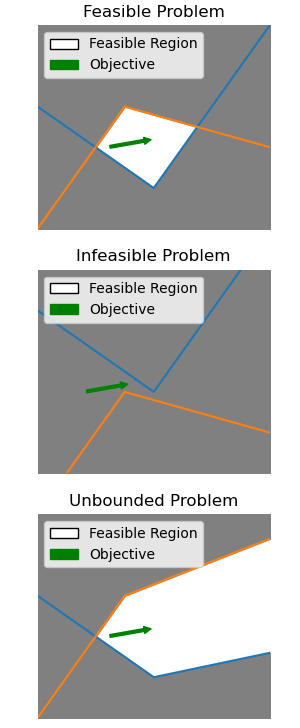
\includegraphics[width=\linewidth]{InfeasibleUnbounded.png}
            \end{figure}
        \end{column}
    \end{columns}
\end{frame}

\begin{frame}{Handling Unbounded Problems}
    \begin{itemize}
        \item Recall that a problem will be unbounded if there are no bounds on the values that certain variables can take on.
        \item Thus, \textbf{imposing an artificial bound on key variables} can cause an unbounded problem to become bounded.
        \item When defining a variable, including a bound on each variable that is \textbf{so big that it would be noticeably too big} (but technically not infinity) could solve this problem.
        \begin{itemize}
            \item Example: If I'm maximizing revenue, if I say that revenue must be between -\$1,000,000,000 and \$1,000,000,000 then the problem would no longer be unbounded.
        \end{itemize}
        \item One word of caution: Computers have a hard time with REALLY REALLY large numbers and it might crash if you enter a number absurdly big.
        \item I suggest thinking of the biggest reasonable quantity that that variable should have, and multiplying by 10.
    \end{itemize}
    \hrule
    \vspace{-0.3cm}
    \begin{columns}
        \begin{column}{0.00\textwidth}
            
        \end{column}
        \begin{column}{0.8\textwidth}
            \begin{enumerate}
                \item With this new bound, if you re-solve the solver should at least give you a solution.
                \item Inspect this solution to see which variables are unreasonably large and why.
                \item Add a new constraint and/or bound as needed.
            \end{enumerate}
        \end{column}
        \begin{column}{0.2\textwidth}
            \begin{figure}
                \includegraphics[width=0.9\linewidth]{NotUnbounded.png}
            \end{figure}
        \end{column}
    \end{columns}
\end{frame}

\begin{frame}{Handling Infeasible Problems}
    \begin{itemize}
        \item Recall that a problem will be infeasible if two or more constraints make it so that no possible solution can satisfy all of them.
        \item There are 3 approaches (that I'm familiar with) to address this:
        \begin{enumerate}
            \item Sequentially remove constraints until the problem is no longer infeasible
            \item If you know a feasible solution, enter it and observe which constraints it violates.
            \item Slightly modify the problem to quantify \textbf{just how infeasible} a solution is. Minimize this infeasibility.
        \end{enumerate}
        \item Next we'll go over each of these approaches along with their pros and cons.
    \end{itemize}
\end{frame}

\begin{frame}{Infeasible: Sequentially Remove Constr.}
    \vspace{-0.4cm}
    \begin{columns}
        \begin{column}{0.5\textwidth}
            \begin{enumerate}
                \item Remove a constraint.
                \item Re-optimize.
                \item If still infeasible, remove another.
                \item If not infeasible, you know that (at least one of) the constraint(s) is causing the issue.
                \begin{itemize}
                    \item Go look at those constraints. Are they coded right? Do they make sense?
                \end{itemize}
                \item Repeat (potentially trying different combinations of constraints to see which combination causes the issue).
            \end{enumerate}
            \hrule
            \vspace{0.1cm}
            EXAMPLE:
            \begin{tabular}{|c|c|c||c|}
                \hline
                C1 & C2 & C3 & Feasible? \\
                \hline \hline
                \cmark & \cmark & \cmark & \xmark \\
                \xmark & \cmark & \cmark & \xmark \\
                \xmark & \xmark & \cmark & \cmark \\
                \cmark & \xmark & \cmark & \cmark \\
                \cmark & \cmark & \xmark & \cmark \\
                \hline
            \end{tabular}
        \end{column}
        \begin{column}{0.5\textwidth}
            The Gist: \textbf{Easiest but the least reliable approach.}
            \vspace{0.3cm}
            \begin{itemize}
                \item PROS:
                \begin{itemize}
                    \item Very easy to do (just comment-out constraints).
                    \item You don't need any additional information or re-formulation.
                \end{itemize}
                \item CONS:
                \begin{itemize}
                    \item You technically need to try every possible combination in order to prove where the problem is happening.
                    \item Often when you remove a constraint, an infeasible solution can turn into an unbounded solution.
                \end{itemize}
            \end{itemize}
        \end{column}
    \end{columns}
\end{frame}

\begin{frame}{Infeasible: Known Solution}
    \begin{columns}
        \begin{column}{0.5\textwidth}
            \begin{enumerate}
                \item Insert a known feasible solution into the model.
                \item Iterate over all the constraints to determine which ones are violated by this solution.
                \item Those constraints must be coded and/or ideologically incorrect.
            \end{enumerate}
            \hrule
            \vspace{0.1cm}
            \begin{itemize}
                \item PROS:
                \begin{itemize}
                    \item Guaranteed to work.
                \end{itemize}
                \item CONS:
                \begin{itemize}
                    \item Requires you to know of and be able to insert a known solution.
                \end{itemize}
            \end{itemize}
            
        \end{column}
        \begin{column}{0.5\textwidth}
            The Gist: \textbf{Best approach if you have a known solution (or one is easy to generate).}
            \begin{itemize}
                \item Inserting a known solution, iterating over constraints, and testing feasibility are somewhat nontrivial in Pyomo.
                \item I've made some tools to automate this process:
            \end{itemize}
            \begin{figure}
                \includegraphics[width=\linewidth]{KnownSolutionWorkflow.png}
            \end{figure}
        \end{column}
    \end{columns}
\end{frame}

\begin{frame}{Infeasible: Minimize Infeasibility}
    \begin{columns}
        \begin{column}{0.5\textwidth}
            \begin{enumerate}
                \item Re-formulate the problem using non-negative auxiliary variables to eliminate the possibility of an infeasible solution.
                \item Define a new objective to minimize these aux. vars.
                \item Optimize the re-formulated model.
                \item Any constraints with non-zero aux. vars. are incompatible with other constraints that have non-zero aux. vars.
            \end{enumerate}
            \hrule
            \vspace{0.1cm}
            \begin{itemize}
                \item Equality Constraint: Add an aux. var. to both sides.
                \item $\leq$ Constraint: Add an aux. var. to the right-hand-side.
                \item $\geq$ Constraint: Add an aux. var. to the left-hand-side.
            \end{itemize}
        \end{column}
        \begin{column}{0.5\textwidth}
            The Gist: \textbf{Think of this as the automated version of approach #1.}
            \begin{itemize}
                \item PROS:
                \begin{itemize}
                    \item Is a bit more rigorous/thorough than approach #1.
                    \item Doesn't require a known solution.
                \end{itemize}\item CONS:
                \begin{itemize}
                    \item Requires the computer to solve a separate (potentially very difficult) optimization problem.
                    \item Can require a lot of work to reformulate. I've automated the process for you:
                \end{itemize}
            \end{itemize}
            \begin{figure}
                \includegraphics[width=\linewidth]{FindLeastInfeasibleSolution.png}
            \end{figure}
        \end{column}
    \end{columns}
\end{frame}

\begin{frame}{Conclusion}
    \begin{itemize}
        \item Debugging can be a long, tedious, frustrating, and unavoidable process. 
        \begin{itemize}
            \item Even professionals software engineers can spend up to 50\% of their time debugging.
        \end{itemize}
        \item I'd suggest testing your code \textbf{frequently AS YOU WRITE IT}.
        \begin{itemize}
            \item Don't wait till you're done with the whole problem to try to run your code.
            \item The closer you can narrow down the source of a problem the faster.
        \end{itemize}
        \vspace{0.5cm}
        \item You won't always have a teacher or classmates to depend on.
        \begin{itemize}
            \item One resource you will always have: \textbf{The Internet!}
            \item Asking Google (or ChatGPT) about your problem is often very effective.
            \item Easy, free, and effective place to find ChatGPT: https://copilot.microsoft.com
        \end{itemize}
        \item If you can get good at this, you'll do well as an independent programmer.
    \end{itemize}
\end{frame}

\end{document}